\chapter{Materiais e Métodos}
\label{c3}


A produção de \textit{clusters} é suportada basicamente por duas técnicas: \textit{top-down} e \textit{bottom-up}. Na primeira, a partir de um material com dimensões macroscópicas, as nanoestruturas são formadas a partir da remoção deste material utilizando técnicas como feixe de elétrons ou litografia de feixe de íons focalizado. Na segunda técnica, as nanopartículas são produzidas por síntese química, e então a organização entre elas se da por propriedades físicas ou químicas.

A produção de nanopartículas por síntese química é mais simples porém o controle de pureza torna-se mais complicado. O método de produção por síntese física (\textit{top-down}), requer um aparato experimental sofisticado, que será apresentado neste capítulo, porém o controle de pureza dos \textit{clusters} é altamente preciso.





\section{A Fonte de \textit{Clusters} e Agregados}

A Fonte de \textit{Clusters} e Agregados (FoCA), esquematizada na Figura \ref{fig:esquema_foca}, produz nanopartículas metálicas que variam entre $1$ podendo chegar $40.000$ átomos (ou $5nm$, no caso da prata), essa produção se da por método físico, mais especificamente \textit{sputtering}.

O funcionamento da máquina ocorre basicamente em quatro etapas: primeiramente uma nuvem de átomos é produzida por um \textit{sputtering}; em seguida, são resfriadas por nitrogênio líquido ocorrendo a agregação dos átomos em nanopartículas na presença do gás argônio; na sequência, o feixe de agregados, carregados eletricamente, é guiado por um conjunto de lentes eletrostáticas até chegar no espectrômetro de massa por tempo de voo, onde $\approx10\%$ do feixe é desviado para a análise do espectro de distribuição de massa, sendo possível identificar a massa e por consequência o tamanho das partículas produzidas, por fim as nanopartículas são depositadas no porta amostras. Na Figura \ref{fig:foto_foca} podemos ver uma foto real da máquina. 

\begin{figure}
  \centering
  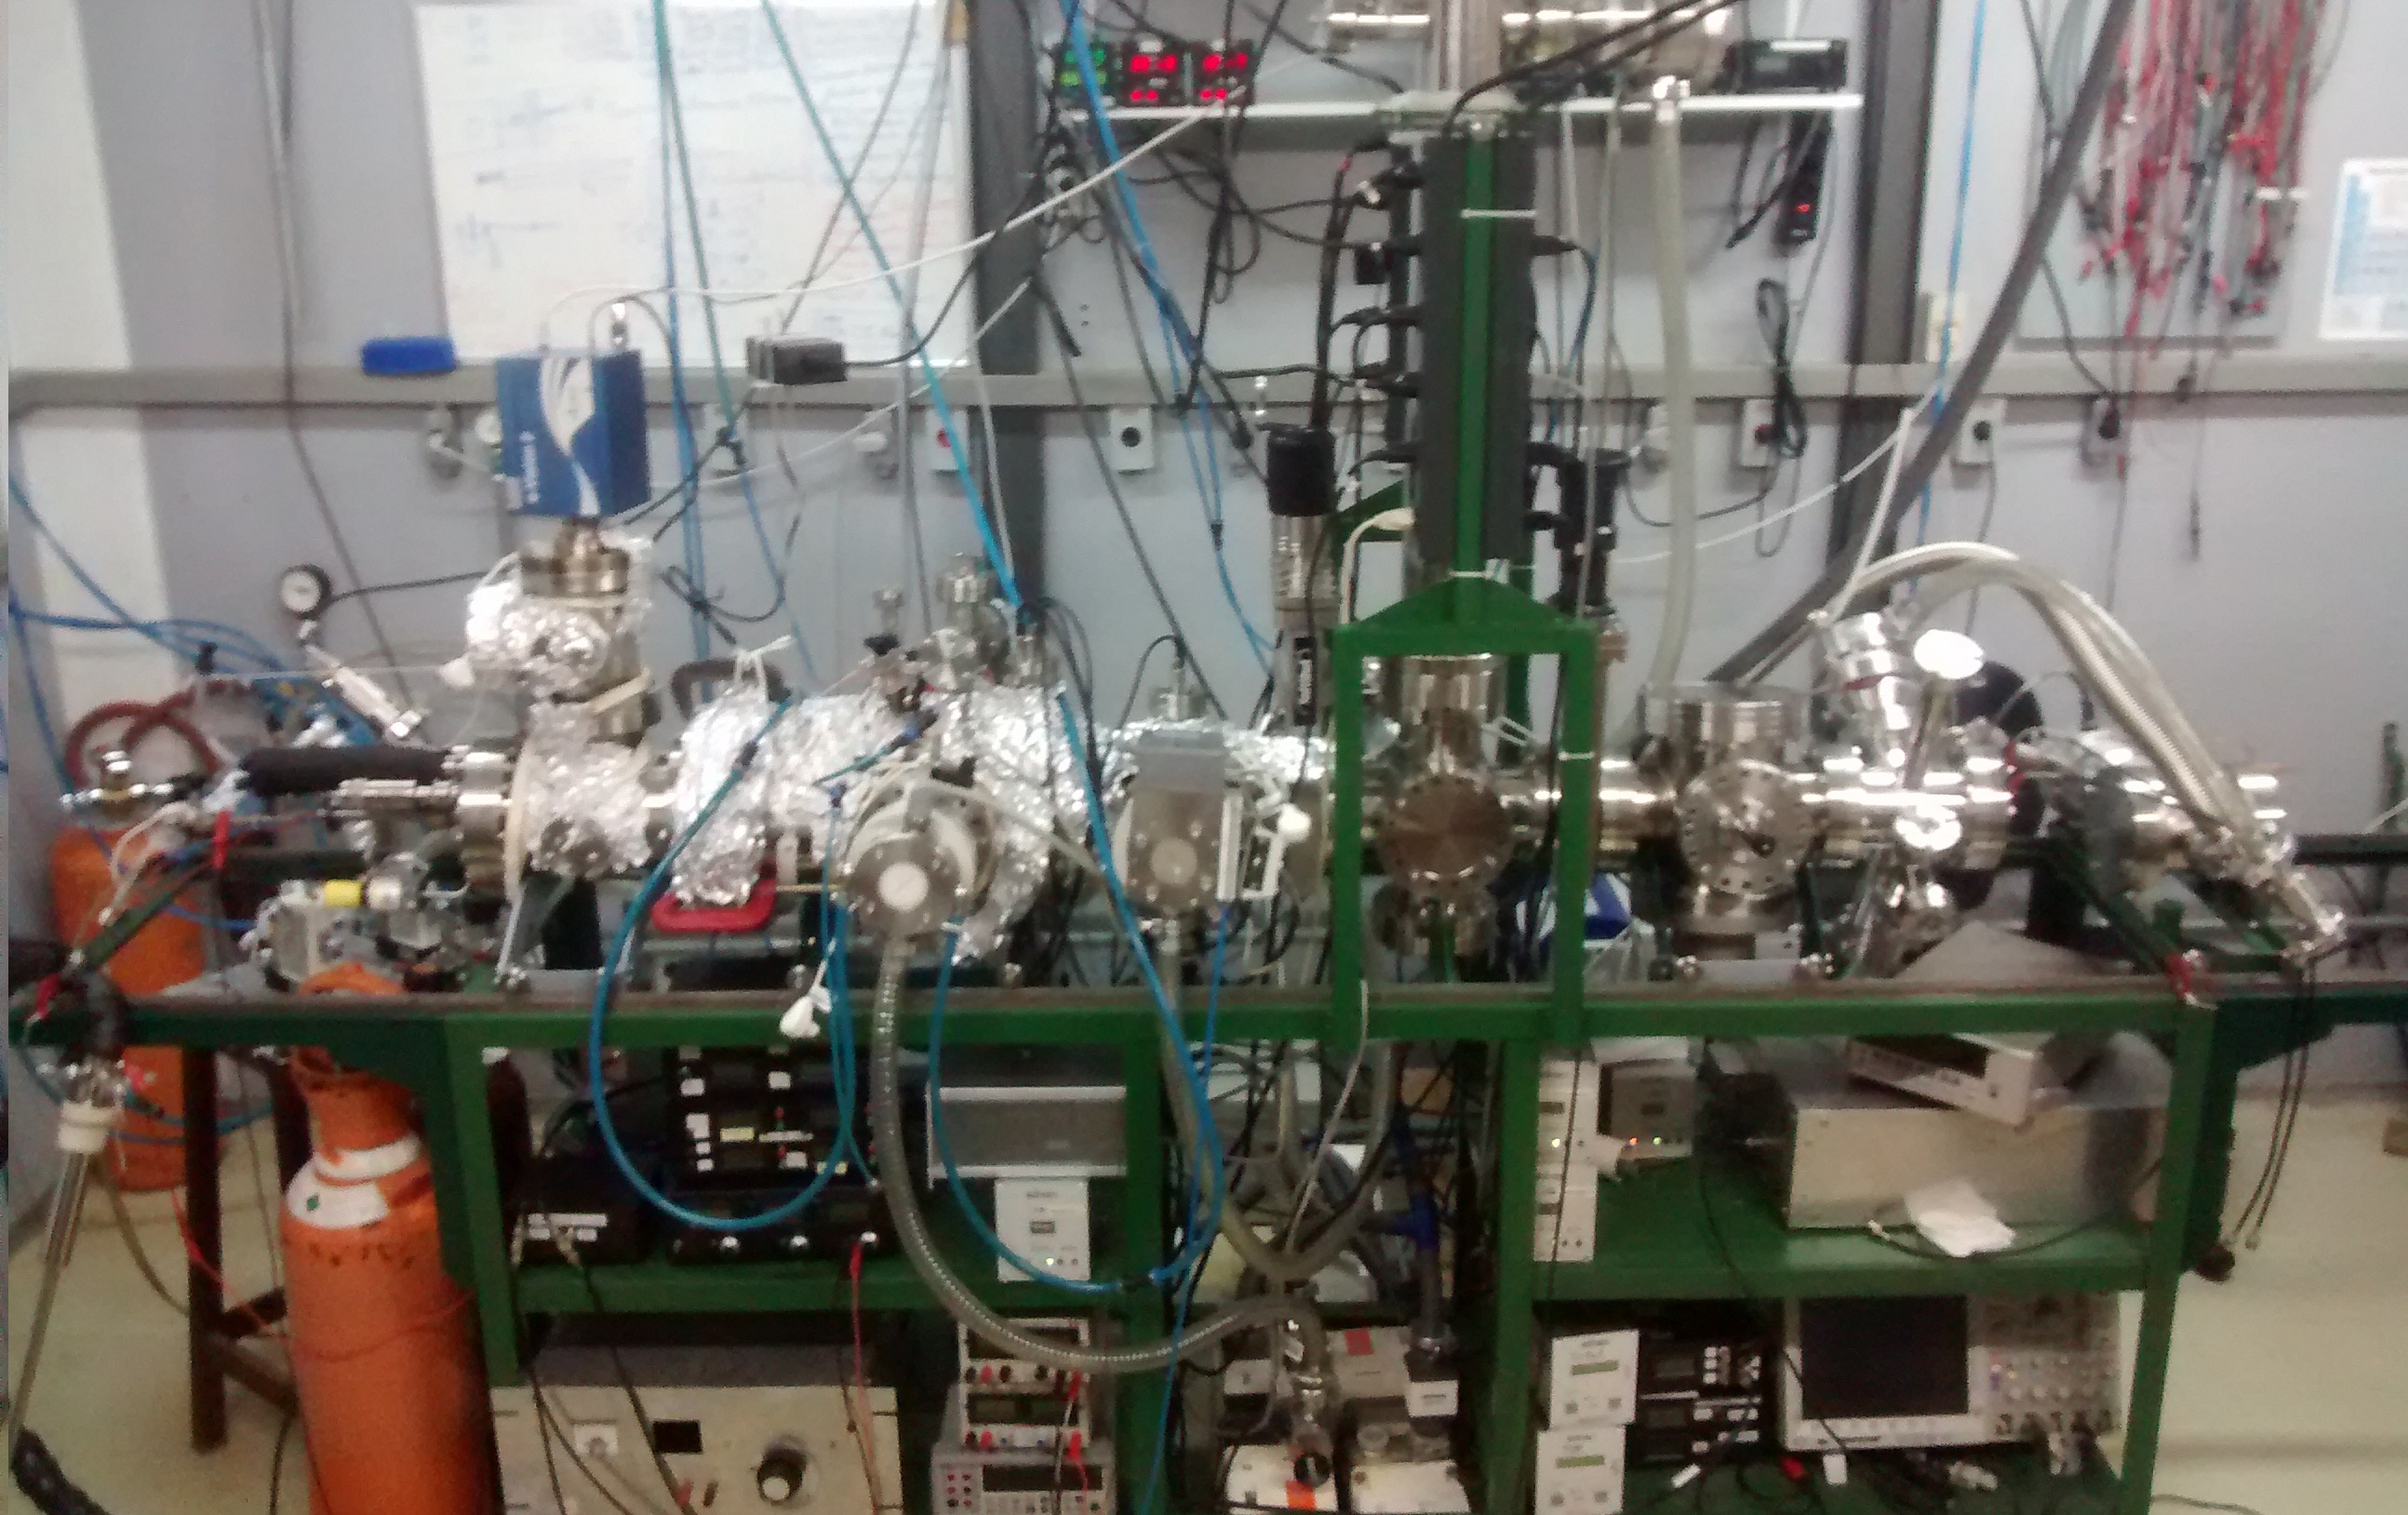
\includegraphics[width=0.7\textwidth]{images/foca/foto_foca}
  \caption{ Imagem real da  Fonte de \textit{Clusters} e Agregados.  }
  \label{fig:foto_foca}
\end{figure}

\begin{figure}
  \centering
  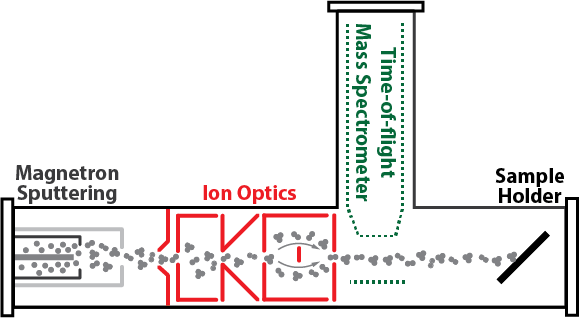
\includegraphics[width=0.8\textwidth]{images/foca/esquematico_foca}
  \caption{ Diagrama da fonte de Fonte de \textit{Clusters} e Agregados. ``\textit{Magnetron Sputtering}'' é a fonte de átomos que se encontra dentro da câmara de agregação. Depois de produzido e agregado, o feixe passa por um conjunto de lentes eletrostásticas  ``\textit{Ion Optics}''. Uma parte do feixe é desviado para o ``\textit{Time-of-flight Mass Spectrometers}'' (ToF), onde é realizada a aquisição do espectro de voo, outra parte é depositada na amostra "\textit{Sample Holder}"\cite{livro_vitor}.  }
  \label{fig:esquema_foca}
\end{figure}

As lentes eletrostáticas possuem as seguintes funções: focalizar o feixe de íons, retirar as partículas neutras, de acordo com o potencial aplicado nas lentes elas também podem funcionar com um filtro em função das energias das partículas. As lentes consistem de uma série de eletrodos de simetria cilíndrica nas quais são aplicadas potenciais. Uma foto das lentes pode ser vista na Figura \ref{fig:foto_lentes}.

\begin{figure}
  \centering
  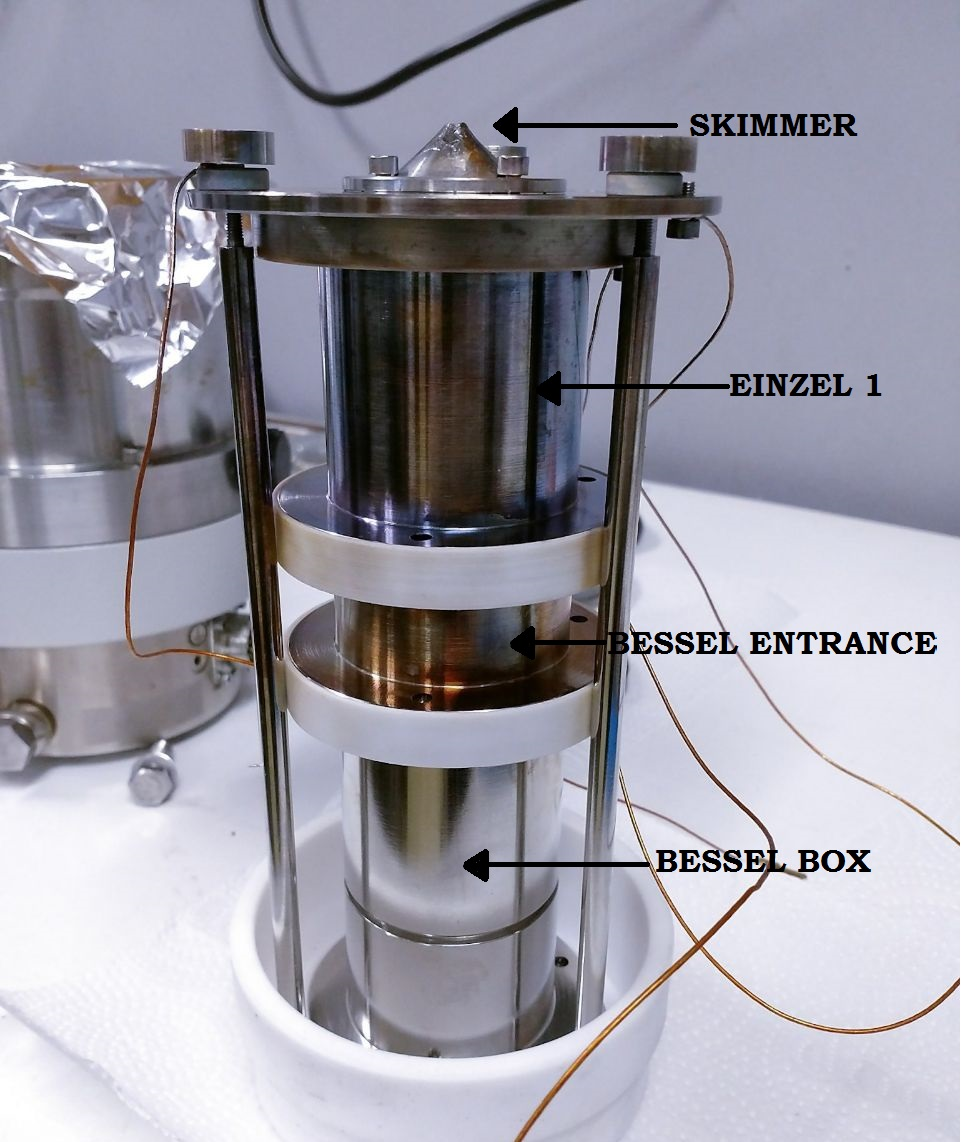
\includegraphics[width=0.6\textwidth]{images/foca/lentes}
  \caption{ Foto da lentes eletrostáticas.  }
  \label{fig:foto_lentes}
\end{figure}



Existem muitas formas de síntese de nanopartículas, seja por método químico ou físico. Como exemplo da primeira, para o caso da prata, podemos citar a redução com borohidreto de sódio e como exemplo da segunda, agora em um caso mais geral de metais, podemos citar a evaporação térmica e a técnica de \textit{sputtering} ou pulverização catódica.

Para gerar nossa nuvem de átomos, a FoCA utiliza um \textit{magnetron cilíndrico} \cite{ref_artigo_foca}, que caracteriza a produção desses \textit{clusters} por \textit{sputtering}, aqui o alvo, material que dará origem às nanopartículas, possuí o formato de um fio e fica localizado no eixo do \textit{magnetron}.

A versatilidade dessa técnica encontra-se no fato que o alvo é multivalente, podendo ser composto de vários metais, incluindo ligas, como por exemplo a mistura ouro e prata, bastando entrelaçar os fios do metal de desejo para isso. Na Figura \ref{fig:magnetron} podemos ver o plasma gerado no \textit{magnetron cilíndrico}. Pela presença de um campo elétrico os íons são acelerados em direção ao alvo do metal de interesse e o corrói. Na Figura \ref{fig:alvo} é possível observar um alvo de prata, composto por um único fio, novo e ao lado um já erodido.

\begin{figure}
  \centering
  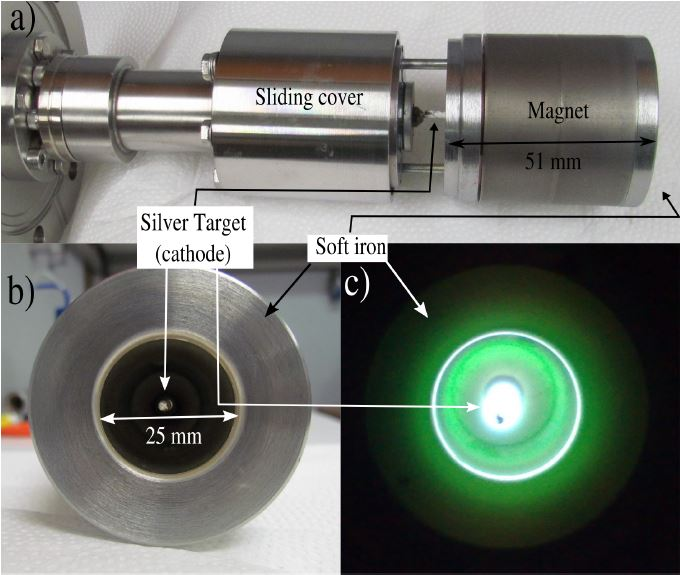
\includegraphics[width=0.75\textwidth]{images/foca/magnetron_cil}
  \caption{ (a) Magnetron cilíndrico oco caseiro com a tampa deslizante retraída para mostrar o alvo de prata. (b) vista frontal. (c) Vista frontal com plasma aberto. Observe a cor esverdeada ao redor do alvo, tipicamente vista na formação de plasma prateado.\cite{livro_vitor} }
  \label{fig:magnetron}  
\end{figure}


\begin{figure}
  \centering
  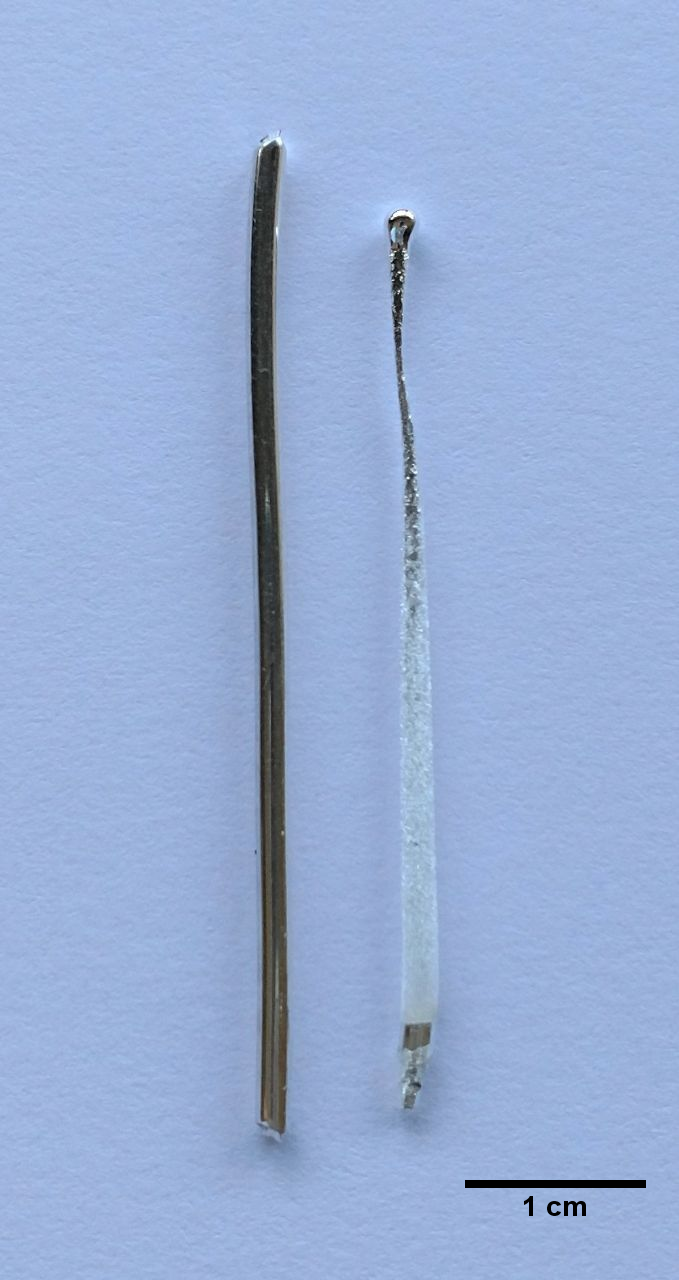
\includegraphics[width=0.3\textwidth]{images/foca/alvo}
  \caption{ Foto de um alvo de prata de fio único. À esquerda temos um alvo novo e à direita temos um alvo já corroído.  }
  \label{fig:alvo}
\end{figure}






\section{Espectrômetro de massa por tempo de voo}

Esta seção será dedicada a descrever o princípio de funcionamento da técnica de \textit{Time-of-flight Mass Spectrometers} (TOFMSs).

Na Figura \ref{fig:tof}, pode-se observar o esquema do espectrômetro, onde o pulso elétrico fornece velocidade perpendicular ao feixe de partículas carregadas, que viajam dentro de um tubo de voo - livre de variação de potencial elétrico - até encontrarem um detetor de corrente. Por sua vez, o detetor faz a contagem de íons em função dos tempos de chegada.

O TOFMSs funciona  baseado no fato de que, ao receber a mesma quantidade de energia fornecida por um campo elétrico pulsado, partículas com massas diferentes adquirem velocidades distintas \cite{dissertacao_kevin}. Assim, as partículas mais leves atingirão o detector antes das partículas mais pesadas.

\begin{figure}
  \centering
  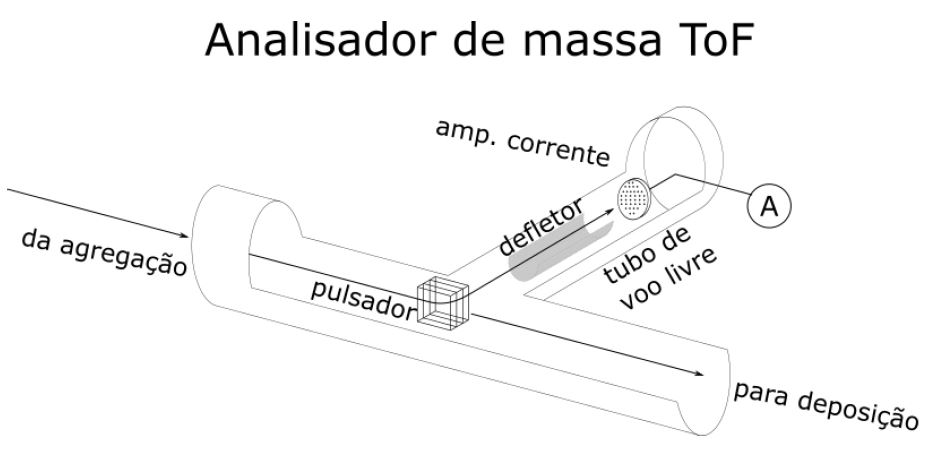
\includegraphics[width=1\textwidth]{images/foca/tof}
  \caption{ O pulsador é um conjunto de placas com campo pulsado, que confere uma velocidade perpendicular ao feixe de partículas eletricamente carregadas. Os defletores impedem que as partículas colidam com as paredes do tubo de voo livre. ``\textit{A}'' representa o detector de corrente, cuja função é realizar a contagem dos íons em função do tempo de chegada.  \cite{dissertacao_kevin}.  }
  \label{fig:tof}
\end{figure}

Para calcular o tempo de voo, vamos considerar um \textit{cluster} de massa $m$ e carga $q$. O campo elétrico vai fornecer energia cinética ($K = qV$) para a partícula, em que $V$ é a voltagem fornecida pelo pulsador. Assim, é possível expressar a velocidade da partícula como:

\begin{equation}
v = \sqrt[]{\frac{2qV}{m}}
\end{equation}

O detector de corrente está situado a uma distância $L$ da região onde a partícula adquire velocidade. Note que essa partícula levará um tempo $t_{voo}$ para atingir o detector, e esse tempo pode ser calculado por:

\begin{equation}
\label{eq:tempo_voo}
t_{voo} = L \cdot \sqrt[]{\frac{1}{2V} \frac{m}{q}} 
\end{equation}


A corrente que chega ao detector é convertida em tensão por um amplificador IV, e o sinal é exibido em um osciloscópio, e então para aquisição dos dados utiliza-se um programa desenvolvido pelo grupo.

A variável $L$ possui o valor de um metro, o potencial aplicado é de $V = 7 $  kV, e o tempo de voo das partículas é fornecido pelo osciloscópio, possibilitando calcular a massa das partículas.

Note que utilizando a Equação \ref{eq:tempo_voo} é possível também calcular o $t_{voo}$ de uma partícula se soubermos a massa. Vamos fazer uma análise para o caso de um átomo de prata. Segundo a tabela periódica um átomo de prata possui uma massa de $107,87$ unidades de massa atômica, convertendo sua massa para quilos temos $1,79\times 10^{-25}$ kg. A carga de partícula é a carga elementar de um elétron $1,60\times 10^{-19}$ C, e então seu tempo de voo vai ser aproximadamente$17,6$ $\mu$s.

Podemos também escrever a massa de uma nanopartícula em função da massa de uma outra partícula da qual conhecemos a massa e o tempo de voo.

\begin{equation}
\label{eq:relacao_massa_tempo}
M = \left(\frac{t}{t'}\right)^2 \cdot M'
\end{equation}


É possível estabelecer uma relação que futuramente vai permitir diferenciar outros picos de prata, e então calibrar o espectro de partículas produzido, confirmando o que foi depositado na amostra.


A grande vantagem desse tipo de técnica, espectrometria de massa por tempo de voo, é que a obtenção da distribuição de tamanhos produzida é exibida em tempo real, assim qualquer deformidade indesejável no espectro é passível de correção ainda durante o processo de deposição, por meio de ajuste  dos parâmetros da máquina. 

\section{Experimentos com luz ultravioleta}

Para realizar experimentos com incidência de luz ultra violeta, foi preciso montar um sistema de iluminação, que consiste em inserir um LED do UV, modelo UVTOP240 TO39 produzido pela Roithner Lasertechnik GmbH, na fonte de agregados. Para isto foi instalado um passante de tensão para que o LED fique em dentro da máquina. Além disso, um sistema de alimentação, com controle de corrente, foi montado utilizando uma fonte de tensão.

O LED é baseados em AlGaN (Alumínio, Gálio e Nitrogênio), com um pico típico de comprimento de onda de $245 nm$ e potência de saída óptica de $30-70 \mu W$. Seu encapsulamento é metálico e hermeticamente fechado, com configuração de lente de vidro plano. Uma foto desse diodo pode ser vista na Figura \ref{fig:foto_led}.

\begin{figure}
  \centering
  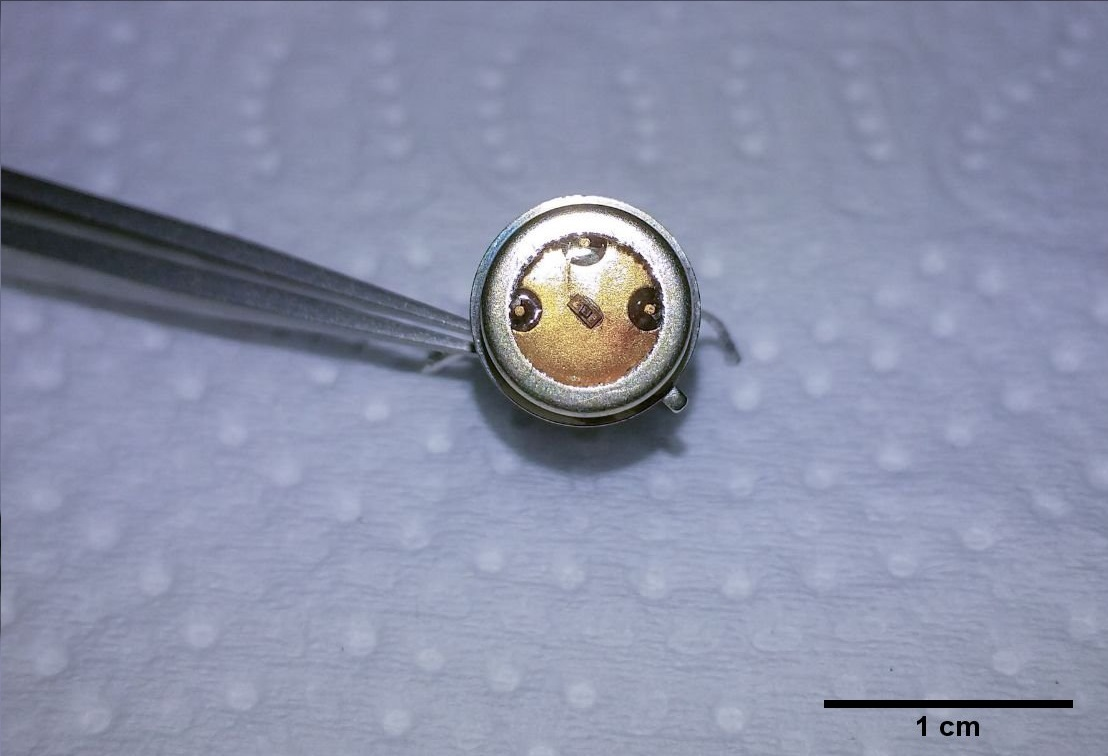
\includegraphics[width=0.7\textwidth]{images/foca/led_scale}
  \caption{ Foto do LED do UV, modelo UVTOP240 TO39, utilizado para ionização das nanopartículas.  }
  \label{fig:foto_led}
\end{figure}


Foi escolhido posicionar o LED entre saída da câmara de agregação e a primeira lente eletrostática, como podemos ver na Figura \ref{fig:led_montagem}. Os testes do aparato consistem na aquisição da corrente de agregados produzidos e do seu espectro de massa sem o uso do LED e posteriormente com o LED. Com isso foi avaliado o possível aumento de ionização, como a incidência de luz afeta o espectro de massa do sistema de agregação e possíveis ajustes nos valores da tensões das lentes eletrostáticas.
Assim, foram realizados experimentos com incidência de luz ultra violeta (UV), induzindo a sua ionização, e comparar os espectros de abundância obtidos com e sem o uso da luz UV. 



\begin{figure}
  \centering
  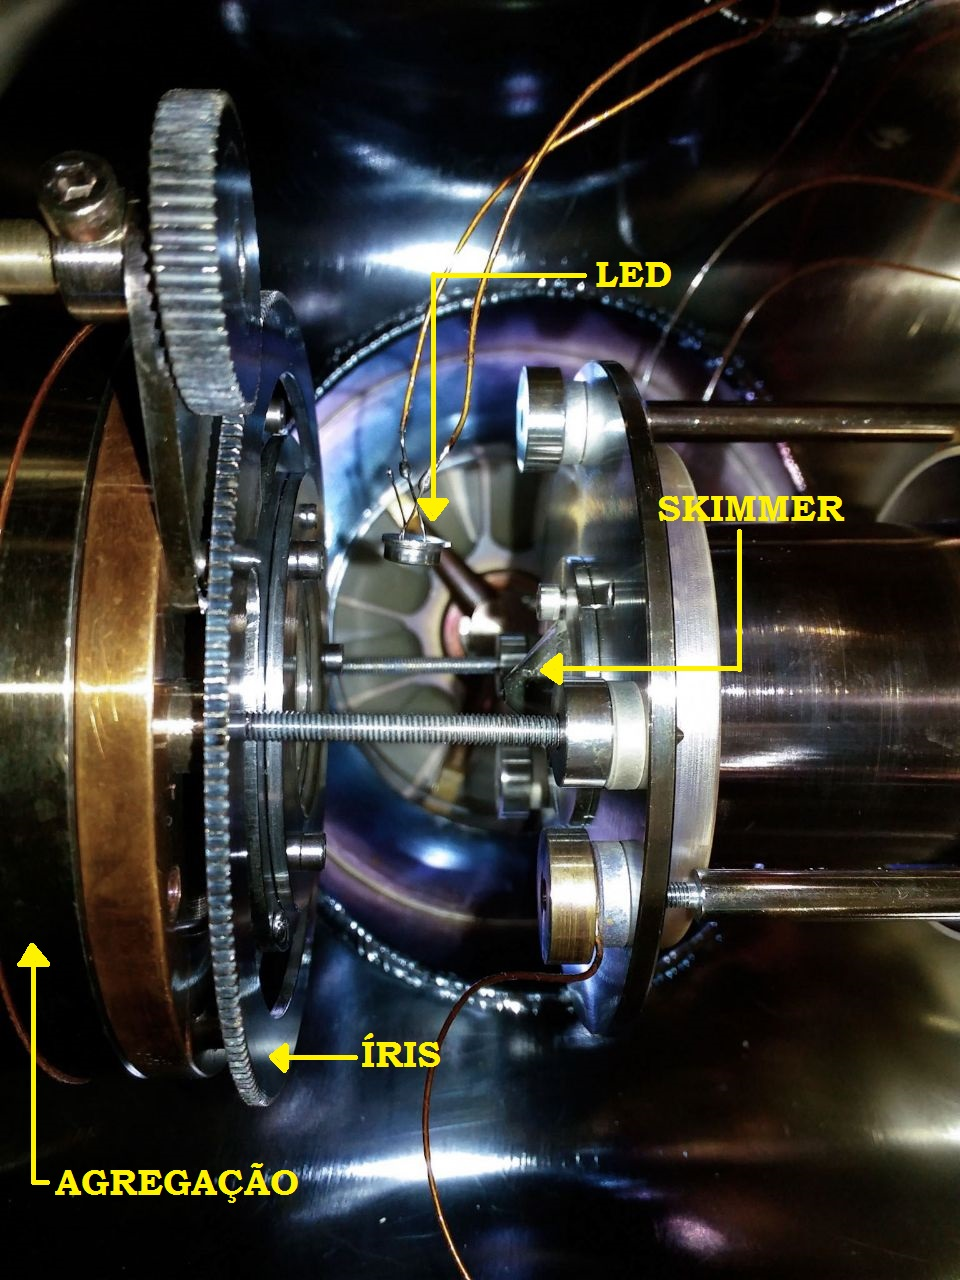
\includegraphics[width=0.7\textwidth]{images/foca/led_montagem}
  \caption{Foto do posicionamento do LED, localizado entre a câmara de deposição e a primeira lente eletrostática, Skimmer. Também está indicado a íris, peça que controla a pressão na câmara de agregação.}
  \label{fig:led_montagem}
\end{figure}


